\chapter{System Design}
This chapter discusses the system design, analysing the various aspects of the project and purpose of each component such as the visualisation, the sorting algorithms, user authentication, the server, etc.

\section{Overview}
\begin{center}
    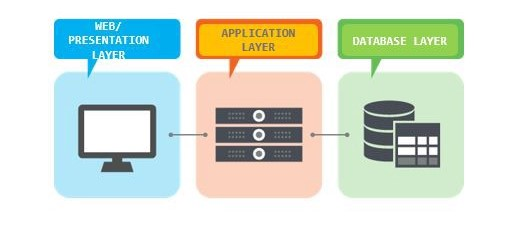
\includegraphics[width=8cm,height=3.3cm,keepaspectratio]{images/3tier}
\end{center}

This project utilises the multi-tier architecture (often referred to as n-tier architecture) platform. Multi-tier architecture or multilayered architecture is a client–server architecture in which presentation, application processing, and data management functions are physically separated. The most widespread use of multi-tier architecture is the three-tier architecture. This project consists of ... main components, all working together: The web application, which represents the presentation layer, allows users to visualise various sorting algorithms, register and login, upload and view past sorts from other users. The Flask server, which represents the logic tier, handles requests such as account registration and log in, and uploading and retrieving of sorts by users.

\begin{center}
    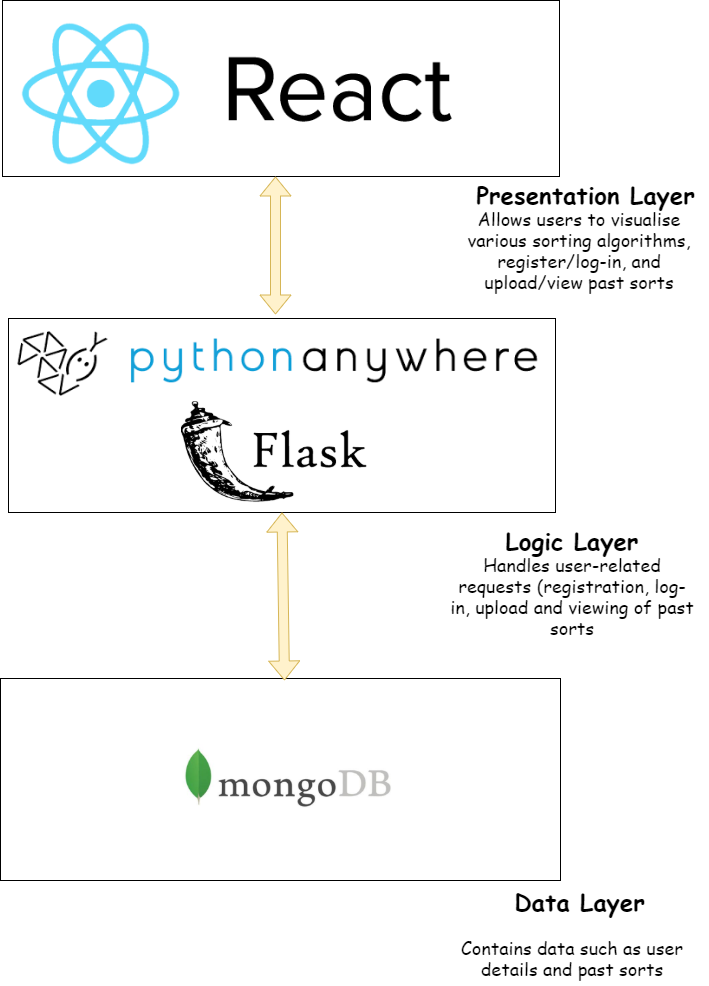
\includegraphics[width=15cm,height=15cm,keepaspectratio]{images/system_design}
\end{center}
\newpage

\section{Web Application}
The web application was designed and developed first as this is the main aspect of the project itself. The main objective of the web application was to allow a user to choose a sorting algorithm and be able to visualise it. Secondary objectives, which were developed at a later point, was to allow users to register and log in to an account, and have the ability to upload and view previous sorts. This was greatly aided by the decision to use ReactJS .... The web application consists of ... main pages: 
\begin{itemize}
    \item \textbf{Sorting Page} - The sorting page is the main page of the application. Allows a user to choose one of several sorting algorithms to visualise, generate a random array of elements to sort, and specify their own dataset to sort.
    \item \textbf{Login Page} - The login page handles user authentication and will login a user to the application if that user exists within the database. The user will then be redirected to the sorting page, with new functionality available such as ...
    \item \textbf{Register Page} - The register page handles user authentication and will register a user with the application. The user will then be redirected to the login page, where they can then attempt to login.
\end{itemize}

\begin{center}
    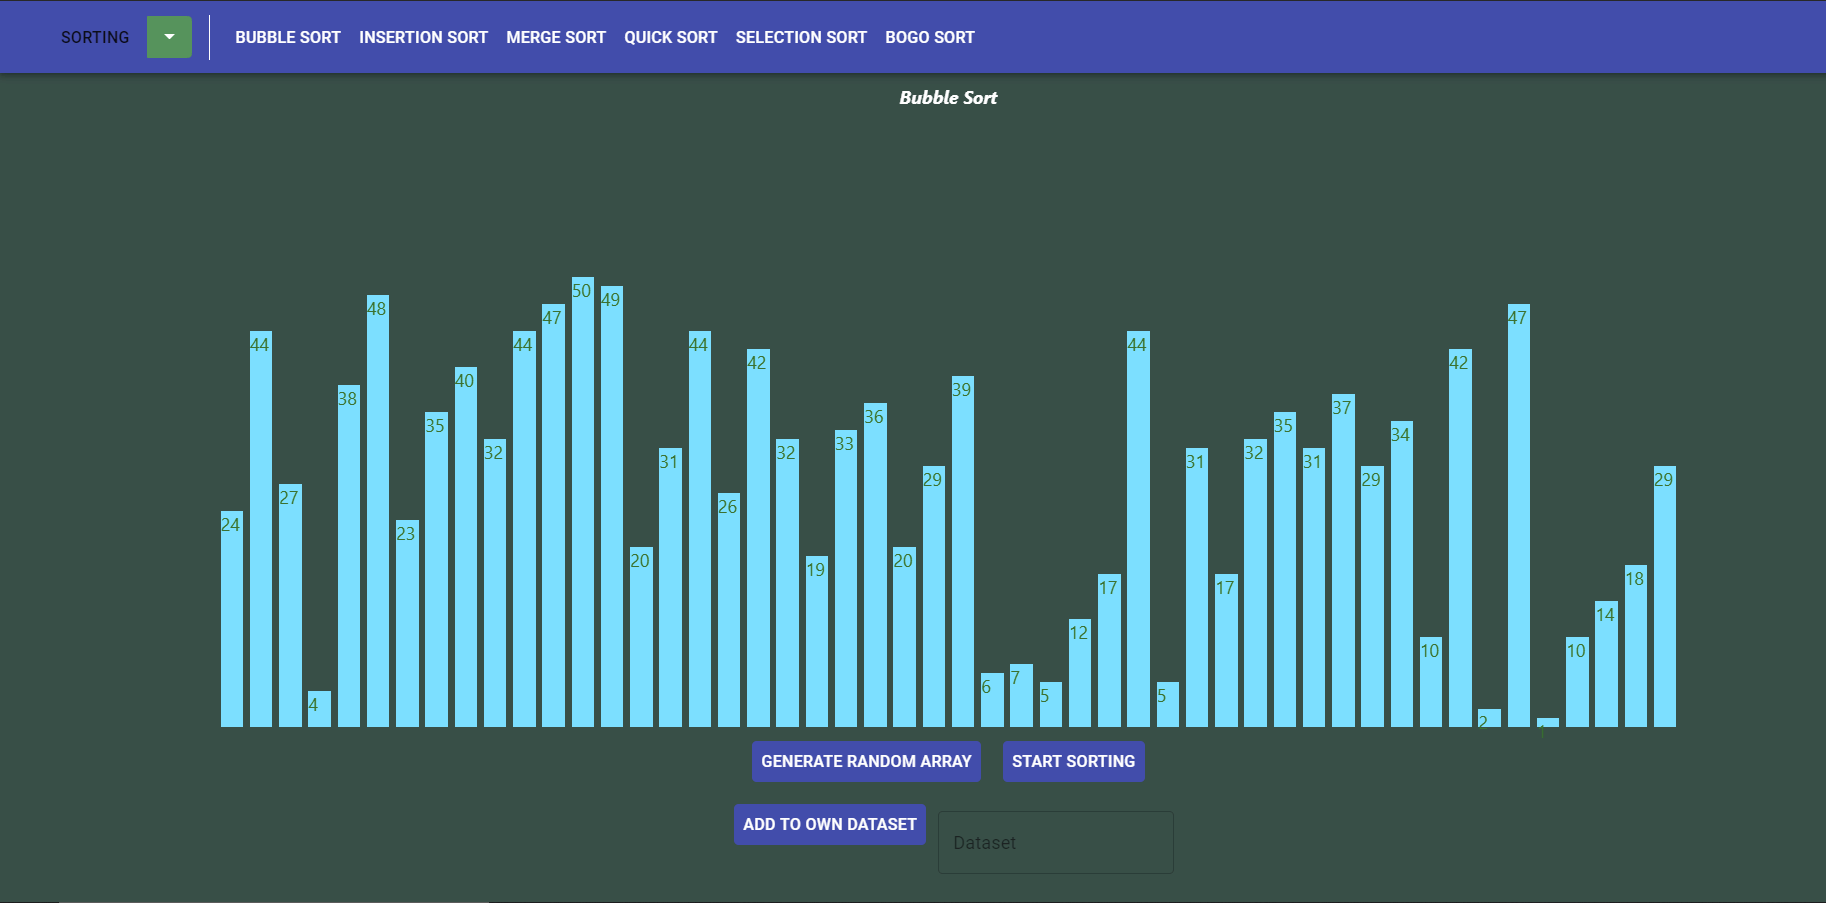
\includegraphics[width=15cm,height=15cm,keepaspectratio]{images/web_app_main}
\end{center}

\section{Flask Server}
The Flask server, which is hosted on PythonAnywhere, is the middle-man of the entire application and allows the web application to communicate with the database. The server was developed and integrated into the web application secondly alongside the database. It handles requests, such as user login requests, user registration requests, uploading saved sorts, etc. made by the web application and performs the appropriate action. The database is then read and/or updated based on this. 

\begin{center}
    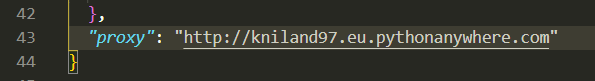
\includegraphics[width=15cm,height=10cm,keepaspectratio]{images/proxy}
    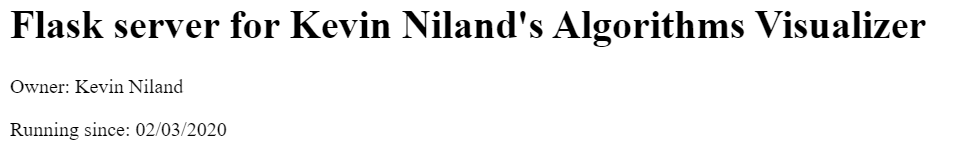
\includegraphics[width=15cm,height=10cm,keepaspectratio]{images/pa_kn}
\end{center}

\section{Database}
The database 